\documentclass{article}
\usepackage{tikz}
\usepackage{parskip}
\usepackage{fullpage}


\title{Tikz Visuals in Latex Assignment}
\author{Steven Rizo}
\date{\vspace{-3ex}}

\begin{document}

\maketitle

\newcommand{\eqncircle}{
	\begin{center}
		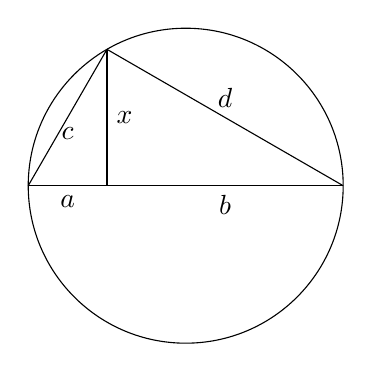
\begin{tikzpicture}
			\draw (2,2) circle (2);
			\draw (0,2) -- node [anchor=north] {$a$} (1,2);
			\draw (1,2) -- node [anchor=north] {$b$} (4,2);
			\draw (1,2) -- node [anchor=west] {$x$} (1,2 + 3^0.5);
			\draw (0,2) -- node [anchor=north] {$c$} (1,2 + 3^0.5);
			\draw (4,2) -- node [anchor=south] {$d$} (1,2 + 3^0.5);
		\end{tikzpicture}
	\end{center}
}

\newcommand{\eqnslope}{
	\begin{center}
		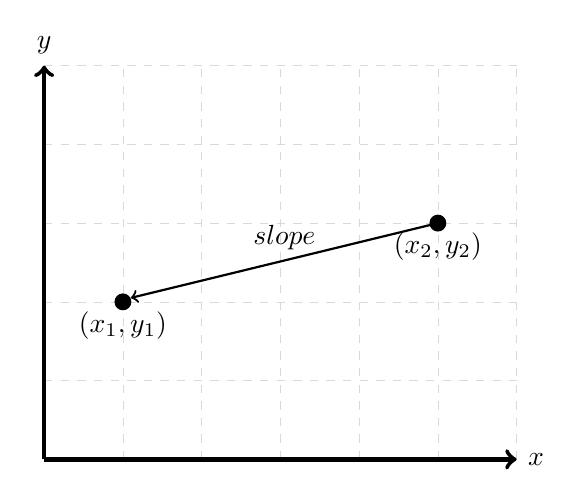
\begin{tikzpicture}
			\draw[help lines, color=gray!30, dashed] (0,0) grid (6,5);
			\draw[->,ultra thick] (0,0)--(6,0) node[anchor=west]{$x$};
			\draw[->,ultra thick] (0,0)--(0,5) node[anchor=south]{$y$};
			\filldraw (1,2) circle (0.1) node[anchor=north]{$(x_1,y_1)$};
			\filldraw (5,3) circle (0.1) node[anchor=north]{$(x_2,y_2)$};
			\draw[->,thick] (5,3)-- node[anchor=south]{$slope$} (1.1,2.05);
		\end{tikzpicture}
	\end{center}
}

Class assigned problem:

\eqncircle{}
\begin{equation}
c^2 + d^2 = (a + b)^2
\end{equation}
\begin{equation}
c^2 = a^2 + x^2
\end{equation}
\begin{equation}
d^2 = b^2 + x^2
\end{equation}

Visual of determining topography from slope:
\eqnslope{}

Arrow indicates direction of positive slope. 

Equation for calculating slope:
\begin{equation}
slope = \frac{y_1 - y_2}{x_1 - x_2}
\end{equation}
Equation to determine new elevation from slope:
\begin{equation}
y_2 = y_1 - slope(x_1 - x_2)
\end{equation}

\end{document}